%*******************************************************************************
%*********************************** Third Chapter *****************************
%*******************************************************************************

\chapter{Probing Correlations by Global 
Nondestructive Addressing} %Title of the Third Chapter

\ifpdf
    \graphicspath{{Chapter3/Figs/Raster/}{Chapter3/Figs/PDF/}{Chapter3/Figs/}}
\else
    \graphicspath{{Chapter3/Figs/Vector/}{Chapter3/Figs/}}
\fi


%********************************** %First Section  **************************************

\section{Introduction}

Having developed the basic theoretical framework within which we can
treat the fully quantum regime of light-matter interactions we now
consider possible applications. There are three prominent directions
in which we can proceed: nondestructive probing of the quantum state
of matter, quantum measurement backaction induced dynamics and quantum
optical lattices. Here, we deal with the first of the three options.

In this chapter we develop a method to measure properties of ultracold
gases in optical lattices by light scattering. In the previous chapter
we have shown that quantum light field couples to the bosons via the
operator $\hat{F}$. This is the key element of the scheme we propose
as this makes it sensitive to the quantum state of the matter and all
of its possible superpositions which will be reflected in the quantum
state of the light itself. We have also shown in section
\ref{sec:derivation} that this coupling consists of two parts, a
density component $\hat{D}$ given by Eq. \eqref{eq:D}, and a phase
component $\hat{B}$ given by Eq. \eqref{eq:B}. Therefore, when probing
the quantum state of the ultracold gas we can have access to not only
density correlations, but also matter-field interference at its
shortest possible distance in an optical lattice, i.e.~the lattice
period. Previous work on quantum non-demolition (QND) schemes
\cite{rogers2014, mekhov2007prl, eckert2008} probe only the density
component as it is generally challenging to couple to the matter-field
observables directly. Here, we will consider nondestructive probing of
both density and interference operators.

Firstly, we will consider the simpler and more typical case of
coupling to the atom number operators via $\hat{F} =
\hat{D}$. However, we show that light diffraction in this regime has
several nontrivial characteristics due to the fully quantum nature of
the interaction. Firstly, we show that the angular distribution has
multiple interesting features even when classical diffraction is
forbidden facilitating their experimental observation. We derive new
generalised Bragg diffraction conditions which are different to their
classical counterpart. Furthermore, due to the fully quantum nature of
the interaction our proposal is capable of probing the quantum state
beyond mean-field prediction. We demonstrate this by showing that this
scheme is capable of distinguishing all three phases in the Mott
insulator - superfluid - Bose glass phase transition in a 1D
disordered optical lattice which is not very well described by a
mean-field treatment. We underline that transitions in 1D are much
more visible when changing an atomic density rather than for
fixed-density scattering. It was only recently that an experiment
distinguished a Mott insulator from a Bose glass \cite{derrico2014}
via a series of destructive measurements. Our proposal, on the other
hand, is nondestructive and is capable of extracting all the relevant
information in a single experiment.

Having shown the possibilities created by this nondestructive
measurement scheme we move on to considering light scattering from the
phase related observables via the operator $\hat{F} = \hat{B}$. This
enables in-situ probing of the matter-field coherence at its shortest
possible distance in an optical lattice, i.e. the lattice period,
which defines key processes such as tunnelling, currents, phase
gradients, etc. This is in contrast to standard destructive
time-of-flight measurements which deal with far-field interference
although a relatively near-field scheme was use in
Ref. \cite{miyake2011}. We show how within the mean-field treatment,
this enables measurements of the order parameter, matter-field
quadratures and squeezing. This can have an impact on atom-wave
metrology and information processing in areas where quantum optics
already made progress, e.g., quantum imaging with pixellized sources
of non-classical light \cite{golubev2010, kolobov1999}, as an optical
lattice is a natural source of multimode nonclassical matter waves.

\section{Coupling to the Quantum State of Matter}

As we have seen in section \ref{sec:a} under certain approximations
the scattered light mode, $\a_1$, is linked to the quantum state of
matter via 
\begin{equation}
  \label{eq:a-3}
  \a_1 = C \hat{F} = C \left(\hat{D} + \hat{B} \right),
\end{equation}
where the atomic operators $\hat{D}$ and $\hat{B}$, given by
Eq. \eqref{eq:D} and Eq. \eqref{eq:B}, are responsible for the
coupling to on-site density and inter-site interference
respectively. It is crucial to note that light couples to the bosons
via an operator as this makes it sensitive to the quantum state of the
matter as this will imprint the fluctuations in the quantum state of
the scattered light.

Here, we will use this fact that the light is sensitive to the atomic
quantum state due to the coupling of the optical and matter fields via
operators in order to develop a method to probe the properties of an
ultracold gas. Therefore, we neglect the measurement back-action and
we will only consider expectation values of light observables. Since
the scheme is nondestructive (in some cases, it even satisfies the
stricter requirements for a QND measurement \cite{mekhov2012,
  mekhov2007pra}) and the measurement only weakly perturbs the system,
many consecutive measurements can be carried out with the same atoms
without preparing a new sample. We will show how the extreme
flexibility of the the measurement operator $\hat{F}$ allows us to
probe a variety of different atomic properties in-situ ranging from
density correlations to matter-field interference.

\subsection{On-site Density Measurements}

We have seen in section \ref{sec:B} that typically the dominant term
in $\hat{F}$ is the density term $\hat{D}$ \cite{LP2009,
  mekhov2007pra, rist2010, lakomy2009, ruostekoski2009}. This is
simply due to the fact that atoms are localised with lattice sites
leading to an effective coupling with atom number operators instead of
inter-site interference terms. Therefore, we will first consider
nondestructive probing of the density related observables of the
quantum gas. However, we will focus on the novel nontrivial aspects
that go beyond the work in Ref. \cite{mekhov2012, mekhov2007prl,
  mekhov2007pra} which only considered a few extremal cases.

As we are only interested in the quantum information imprinted in the
state of the optical field we will simplify our analysis by
considering the light scattering to be much faster than the atomic
tunnelling. Therefore, our scheme is actually a QND scheme
\cite{rogers2014, mekhov2007prl, mekhov2007pra, eckert2008} as
normally density-related measurements destroy the matter-phase
coherence since it is its conjugate variable, but here we neglect the
$\bd_i b_j$ terms. Furthermore, we will consider a deep
lattice. Therefore, the Wannier functions will be well localised
within their corresponding lattice sites and thus the coefficients
$J_{i,i}$ reduce to $u_1^*(\b{r}_i) u_0(\b{r}_i)$ leading to
\begin{equation}
  \label{eq:D-3}
  \hat{D}=\sum_i^K u_1^*(\b{r}_i) u_0(\b{r}_i) \hat{n}_i,
\end{equation} 
which for travelling
[$u_l(\b{r})=\exp(i \b{k}_l \cdot \b{r}+i\varphi_l)$] or standing
[$u_l(\b{r})=\cos(\b{k}_l \cdot \b{r}+\varphi_l)$] waves is just a
density Fourier transform at one or several wave vectors
$\pm(\b{k}_1 \pm \b{k}_0)$. 

We will now define a new auxiliary quantity to aid our analysis,
\begin{equation}
  \label{eq:R}
  R = \langle \ad_1 \a_1 \rangle - | \langle \a_1 \rangle |^2,
\end{equation}
which we will call the ``quantum addition'' to light scattering. By
construction $R$ is simply the full light intensity minus the
classical field diffraction. In order to justify its name we will show
that this quantity depends purely quantum mechanical properties of the
ultracold gase. We will substitute $\a_1 = C \hat{D}$ using
Eq. \eqref{eq:D-3} into our expression for $R$ in Eq. \eqref{eq:R} and
we will make use of the shorthand notation
$A_i = u_1^*(\b{r}_i) u_0(\b{r}_i)$. The result is
\begin{equation}
  R = |C|^2 \sum_{i,j}^K A^*_i A_j \langle \delta \hat{n}_i \delta
  \hat{n}_j \rangle,
\end{equation}
where $\delta \hat{n}_i = \hat{n}_i - \langle \hat{n}_i
\rangle$. Thus, we can clearly see that $R$ is a result of light
scattering from fluctuations in the atom number which is a purely
quantum mechanical property of a system. Therefore, $R$, the ``quantum
addition'' faithfully represents the new contribution from the quantum
light-matter interaction to the diffraction pattern.

If instead we are interested in quantities linear in $\hat{D}$, we can
measure the quadrature of the light fields which in section
\ref{sec:a} we saw that $\hat{X}_\phi = |C| \hat{X}^F_\beta$. For the
case when both the scattered mode and probe are travelling waves the
quadrature
\begin{equation} 
  \hat{X}^F_\beta = \frac{1}{2} \left( \hat{F} e^{-i \beta} +
    \hat{F}^\dagger e^{i \beta} \right) = \sum_i^K \hat{n}_i\cos[(\b{k}_1 - \b{k}_2) \cdot
  \b{r}_i - \beta].
\end{equation} 
Note that different light quadratures are differently coupled to the
atom distribution, hence by varying the local oscillator phase, and
thus effectively $\beta$, and/or the detection angle one can scan the
whole range of couplings. A similar expression exists for $\hat{D}$
for a standing wave probe, where $\beta$ is replaced by $\varphi_0$,
and scanning is achieved by varying the position of the wave with
respect to atoms.

The ``quantum addition'', $R$, and the quadrature variance,
$(\Delta X^F_\beta)^2$, are both quadratic in $\a_1$. Therefore, they
will havea nontrivial angular dependence, showing more peaks than
classical diffraction. Furthermore, these peaks can be tuned very
easily with $\beta$ or $\varphi_l$. Fig. \ref{fig:scattering} shows
the angular dependence of $R$ for the case when the scattered mode is
a standing wave and the probe is a travelling wave scattering from
bosons in a 3D optical lattice. The first noticeable feature is the
isotropic background which does not exist in classical
diffraction. This background yields information about density
fluctuations which, according to mean-field estimates (i.e.~inter-site
correlations are ignored), are related by
$R = K( \langle \hat{n}^2 \rangle - \langle \hat{n} \rangle^2 )/2$. In
Fig. \ref{fig:scattering} we can see a significant signal of
$R = |C|^2 N_K/2$, because it shows scattering from an ideal
superfluid which has significant density fluctuations with
correlations of infinte range. However, as the parameters of the
lattice are tuned across the phase transition into a Mott insulator
the signal goes to zero. This is because the Mott insulating phase has
well localised atoms at each site which suppresses density
fluctuations entirely leading to absolutely no ``quantum addition''.

\begin{figure}[htbp!]
  \centering
  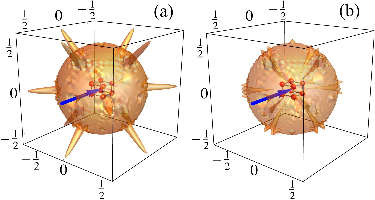
\includegraphics[width=\linewidth]{Ep1}
  \caption[Light Scattering Angular Distribution]{Light intensity
    scattered into a standing wave mode from a superfluid in a 3D
    lattice (units of $R/(|C|^2N_K)$). Arrows denote incoming
    travelling wave probes. The classical Bragg condition,
    $\Delta \b{k} = \b{G}$, is not fulfilled, so there is no classical
    diffraction, but intensity still shows multiple peaks, whose
    heights are tunable by simple phase shifts of the optical beams:
    (a) $\varphi_1=0$; (b) $\varphi_1=\pi/2$. Interestingly, there is
    also a significant uniform background level of scattering which
    does not occur in its classical counterpart. }
  \label{fig:scattering}
\end{figure}

We can also observe maxima at several different angles in
Fig. \ref{fig:scattering}. Interestingly, they occur at different
angles than predicted by the classical Bragg condition. Moreover, the
classical Bragg condition is actually not satisfied which means there
actually is no classical diffraction on top of the ``quantum
addition'' shown here. Therefore, these features would be easy to see
in an experiment as they wouldn't be masked by a stronger classical
signal.  We can even derive the generalised Bragg conditions for the
peaks that we can see in Fig. \ref{fig:scattering}. 

% Derive and show these Bragg conditions

As $(\Delta X^F_\beta)^2$ and $R$ are quadratic variables,
the generalized Bragg conditions for the peaks are
$2 \Delta \b{k} = \b{G}$ for quadratures of travelling waves, where
$\Delta \b{k} = \b{k}_0 - \b{k}_1$ and $\b{G}$ is the reciprocal
lattice vector, and $2 \b{k}_1 = \b{G}$ for standing wave $\a_1$ and
travelling $\a_0$, which is clearly different from the classical Bragg
condition $\Delta \b{k} = \b{G}$. The peak height is tunable by the
local oscillator phase or standing wave shift as seen in Fig.
\ref{fig:scattering}b.

In section \ref{sec:Efield} we have estimated the mean photon
scattering rates integrated over the solid angle for the only two
experiments so far on light diffraction from truly ultracold bosons
where the measurement object was light
\begin{equation} 
  n_{\Phi}= \left(\frac{\Omega_0}{\Delta_a}\right)^2 \frac{\Gamma K}{8}
  (\langle\hat{n}^2\rangle-\langle\hat{n}\rangle^2).
\end{equation} 
Therefore, applying these results to the scattering patters in
Fig. \ref{fig:scattering} the background signal should reach
$n_\Phi \approx 10^6$ s$^{-1}$ in Ref. \cite{weitenberg2011} (150
atoms in 2D), and $n_\Phi \approx 10^{11}$ s$^{-1}$ in
Ref. \cite{miyake2011} ($10^5$ atoms in 3D). These numbers show that
the diffraction patterns we have seen due to the ``quantum addition''
should be visible using currently available technology, especially
since the most prominent features, such as Bragg diffraction peaks, do
not coincide at all with the classical diffraction pattern.

\subsection{Mapping the quantum phase diagram}

\begin{figure}[htbp!]  
  \centering
  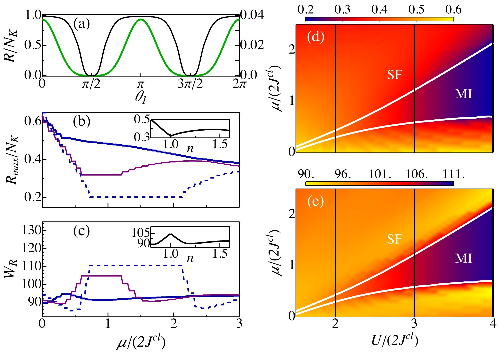
\includegraphics[width=\linewidth]{oph11}
  \caption[Mapping the Bose-Hubbard Phase Diagram]{(a) The angular
    dependence of scattered light $R$ for a superfluid (thin black,
    left scale, $U/2J^\text{cl} = 0$) and Mott insulator (thick green,
    right scale, $U/2J^\text{cl} =10$). The two phases differ in both
    their value of $R_\text{max}$ as well as $W_R$ showing that
    density correlations in the two phases differ in magnitude as well
    as extent. Light scattering maximum $R_\text{max}$ is shown in (b,
    d) and the width $W_R$ in (c, e).  It is very clear that varying
    chemical potential $\mu$ or density $\langle n\rangle$ sharply
    identifies the superfluid-Mott insulator transition in both
    quantities. (b) and (c) are cross-sections of the phase diagrams
    (d) and (e) at $U/2J^\text{cl}=2$ (thick blue), 3 (thin purple),
    and 4 (dashed blue). Insets show density dependencies for the
    $U/(2 J^\text{cl}) = 3$ line. $K=M=N=25$.}
	\label{fig:SFMI}
\end{figure}

We have shown how in mean-field, we can track the order parameter,
$\Phi$, by probing the matter-field interference using the coupling of
light to the $\hat{B}$ operator. In this case, it is very easy to
follow the superfluid to Mott insulator quantum phase transition since
we have direct access to the order parameter which goes to zero in the
insulating phase. In fact, if we're only interested in the critical
point, we only need access to any quantity that yields information
about density fluctuations which also go to zero in the MI phase and
this can be obtained by measuring
$\langle \hat{D}^\dagger \hat{D} \rangle$. However, there are many
situations where the mean-field approximation is not a valid
description of the physics. A prominent example is the Bose-Hubbard
model in 1D \cite{cazalilla2011, ejima2011, kuhner2000, pino2012,
  pino2013}. Observing the transition in 1D by light at fixed density
was considered to be difficult \cite{rogers2014} or even impossible
\cite{roth2003}. By contrast, here we propose varying the density or
chemical potential, which sharply identifies the transition. We
perform these calculations numerically by calculating the ground state
using DMRG methods \cite{tnt} from which we can compute all the
necessary atomic observables. Experiments typically use an additional
harmonic confining potential on top of the optical lattice to keep the
atoms in place which means that the chemical potential will vary in
space. However, with careful consideration of the full
($\mu/2J^\text{cl}$, $U/2J^\text{cl}$) phase diagrams in
Fig. \ref{fig:SFMI}(d,e) our analysis can still be applied to the
system \cite{batrouni2002}.

The 1D phase transition is best understood in terms of two-point
correlations as a function of their separation \cite{giamarchi}. In
the Mott insulating phase, the two-point correlations
$\langle \bd_i b_j \rangle$ and
$\langle \delta \hat{n}_i \delta \hat{n}_j \rangle$
($\delta \hat{n}_i =\hat{n}_i-\langle \hat{n}_i\rangle$) decay
exponentially with $|i-j|$. On the other hand the superfluid will
exhibit long-range order which in dimensions higher than one,
manifests itself with an infinite correlation length. However, in 1D
only pseudo long-range order happens and both the matter-field and
density fluctuation correlations decay algebraically \cite{giamarchi}.

The method we propose gives us direct access to the structure factor,
which is a function of the two-point correlation $\langle \delta
\hat{n}_i \delta \hat{n}_j \rangle$, by measuring the light
intensity. For two travelling waves maximally coupled to the density
(atoms are at light intensity maxima so $\hat{F} = \hat{D}$), the
quantum addition is given by
\begin{equation} 
  R =\sum_{i, j} \exp[i (\mathbf{k}_1 - \mathbf{k}_0)
  (\mathbf{r}_i - \mathbf{r}_j)] \langle \delta \hat{n}_i \delta
  \hat{n}_j \rangle,
\end{equation}

The angular dependence of $R$ for a Mott insulator and a superfluid is
shown in Fig. \ref{fig:SFMI}a, and there are two variables
distinguishing the states. Firstly, maximal $R$,
$R_\text{max} \propto \sum_i \langle \delta \hat{n}_i^2 \rangle$,
probes the fluctuations and compressibility $\kappa'$
($\langle \delta \hat{n}^2_i \rangle \propto \kappa' \langle \hat{n}_i
\rangle$).  The Mott insulator is incompressible and thus will have
very small on-site fluctuations and it will scatter little light
leading to a small $R_\text{max}$. The deeper the system is in the MI
phase (i.e. that larger the $U/2J^\text{cl}$ ratio is), the smaller
these values will be until ultimately it will scatter no light at all
in the $U \rightarrow \infty$ limit. In Fig. \ref{fig:SFMI}a this can
be seen in the value of the peak in $R$. The value $R_\text{max}$ in
the SF phase ($U/2J^\text{cl} = 0$) is larger than its value in the MI
phase ($U/2J^\text{cl} = 10$) by a factor of
$\sim$25. Figs. \ref{fig:SFMI}(b,d) show how the value of
$R_\text{max}$ changes across the phase transition. We see that the
transition shows up very sharply as $\mu$ is varied.

Secondly, being a Fourier transform, the width $W_R$ of the dip in $R$
is a direct measure of the correlation length $l$, $W_R \propto
1/l$. The Mott insulator being an insulating phase is characterised by
exponentially decaying correlations and as such it will have a very
large $W_R$. However, the superfluid in 1D exhibits pseudo long-range
order which manifests itself in algebraically decaying two-point
correlations \cite{giamarchi} which significantly reduces the dip in
the $R$. This can be seen in Fig. \ref{fig:SFMI}a and we can also see
that this identifies the phase transition very sharply as $\mu$ is
varied in Figs. \ref{fig:SFMI}(c,e). One possible concern with
experimentally measuring $W_R$ is that it might be obstructed by the
classical diffraction maxima which appear at angles corresponding to
the minima in $R$. However, the width of such a peak is much smaller
as its width is proportional to $1/M$.

It is also possible to analyse the phase transition quantitatively
using our method. Unlike in higher dimensions where an order parameter
can be easily defined within the MF approximation there is no such
quantity in 1D. However, a valid description of the relevant 1D low
energy physics is provided by Luttinger liquid theory
\cite{giamarchi}. In this model correlations in the supefluid phase as
well as the superfluid density itself are characterised by the
Tomonaga-Luttinger parameter, $K_b$. This parameter also identifies
the phase transition in the thermodynamic limit at $K_b = 1/2$. This
quantity can be extracted from various correlation functions and in
our case it can be extracted directly from $R$ \cite{ejima2011}. By
extracting this parameter from $R$ for various lattice lengths from
numerical DMRG calculations it was even possible to give a theoretical
estimate of the critical point for commensurate filling, $N = M$, in
the thermodynamic limit to occur at $U/2J^\text{cl} \approx 1.64$
\cite{ejima2011}. Our proposal provides a method to directly measure
$R$ in a lab which can then be used to experimentally determine the
location of the critical point in 1D.

So far both variables we considered, $R_\text{max}$ and $W_R$, provide
similar information. Next, we present a case where it is very
different. The Bose glass is a localized insulating phase with
exponentially decaying correlations but large compressibility and
on-site fluctuations in a disordered optical lattice. Therefore,
measuring both $R_\text{max}$ and $W_R$ will distinguish all the
phases. In a Bose glass we have finite compressibility, but
exponentially decaying correlations. This gives a large $R_\text{max}$
and a large $W_R$. A Mott insulator will also have exponentially
decaying correlations since it is an insulator, but it will be
incompressible. Thus, it will scatter light with a small
$R_\text{max}$ and large $W_R$. Finally, a superfluid will have long
range correlations and large compressibility which results in a large
$R_\text{max}$ and a small $W_R$.

\begin{figure}[htbp!]  
  \centering
  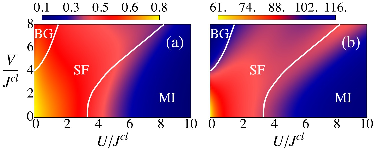
\includegraphics[width=\linewidth]{oph22}
  \caption[Mapping the Disoredered Phase Diagram]{The
    Mott-superfluid-glass phase diagrams for light scattering maximum
    $R_\text{max}/N_K$ (a) and width $W_R$ (b). Measurement of both
    quantities distinguish all three phases. Transition lines are
    shifted due to finite size effects \cite{roux2008}, but it is
    possible to apply well known numerical methods to extract these
    transition lines from such experimental data extracted from $R$
    \cite{ejima2011}. $K=M=N=35$.}
  \label{fig:BG}
\end{figure}

We confirm this in Fig. \ref{fig:BG} for simulations with the ratio of
superlattice- to trapping lattice-period $r\approx 0.77$ for various
disorder strengths $V$ \cite{roux2008}. Here, we only consider
calculations for a fixed density, because the usual interpretation of
the phase diagram in the ($\mu/2J^\text{cl}$, $U/2J^\text{cl}$) plane
for a fixed ratio $V/U$ becomes complicated due to the presence of
multiple compressible and incompressible phases between successive MI
lobes \cite{roux2008}. This way, we have limited our parameter space
to the three phases we are interested in: superfluid, Mott insulator,
and Bose glass. From Fig. \ref{fig:BG} we see that all three phases
can indeed be distinguished. In the 1D BHM there is no sharp MI-SF
phase transition in 1D at a fixed density \cite{cazalilla2011,
  ejima2011, kuhner2000, pino2012, pino2013} just like in
Figs. \ref{fig:SFMI}(d,e) if we follow the transition through the tip
of the lobe which corresponds to a line of unit density. However,
despite the lack of an easily distinguishable critical point it is
possible to quantitatively extract the location of the transition
lines by extracting the Tomonaga-Luttinger parameter from the
scattered light, $R$, in the same way it was done for an unperturbed
BHM \cite{ejima2011}.

Only recently \cite{derrico2014} a Bose glass phase was studied by
combined measurements of coherence, transport, and excitation spectra,
all of which are destructive techniques. Our method is simpler as it
only requires measurement of the quantity $R$ and additionally, it is
nondestructive.

\subsection{Matter-field interference measurements}

We now focus on enhancing the interference term $\hat{B}$ in the
operator $\hat{F}$. 

Firstly, we will use this result to show how one can probe
$\langle \hat{B} \rangle$ which in MF gives information about the
matter-field amplitude, $\Phi = \langle b \rangle$. 

Hence, by measuring the light quadrature we probe the kinetic energy
and, in MF, the matter-field amplitude (order parameter) $\Phi$:
$\langle \hat{X}^F_{\beta=0} \rangle = | \Phi |^2
\mathcal{F}[W_1](2\pi/d) (K-1)$.

Secondly, we show that it is also possible to access the fluctuations
of matter-field quadratures $\hat{X}^b_\alpha = (b e^{-i\alpha} + \bd
e^{i\alpha})/2$, which in MF can be probed by measuring the variance
of $\hat{B}$. Across the phase transition, the matter field changes
its state from Fock (in MI) to coherent (deep SF) through an
amplitude-squeezed state as shown in Fig. \ref{Quads}(a,b). 

Assuming $\Phi$ is real in MF:
\begin{equation}
  \label{intensity} 
  \langle \ad_1 \a_1 \rangle = 2 |C|^2(K-1)\mathcal{F}^2[W_1](\frac{\pi}{d})
  \times [ ( \langle b^2 \rangle - \Phi^2 )^2 + ( n - \Phi^2 ) ( 1 +n - \Phi^2 ) ]
\end{equation} 
and it is shown as a function of $U/(zJ^\text{cl})$ in
Fig. \ref{Quads}. Thus, since measurement in the diffraction maximum
yields $\Phi^2$ we can deduce $\langle b^2 \rangle - \Phi^2$ from the
intensity. This quantity is of great interest as it gives us access to
the quadrature variances of the matter-field
\begin{equation} 
  (\Delta X^b_{0,\pi/2})^2 = 1/4 + [(n - \Phi^2) \pm
  (\langle b^2 \rangle - \Phi^2)]/2,
\end{equation} 
where $n=\langle\hat{n}\rangle$ is the mean on-site atomic density.

\begin{figure}[htbp!]
  \centering
  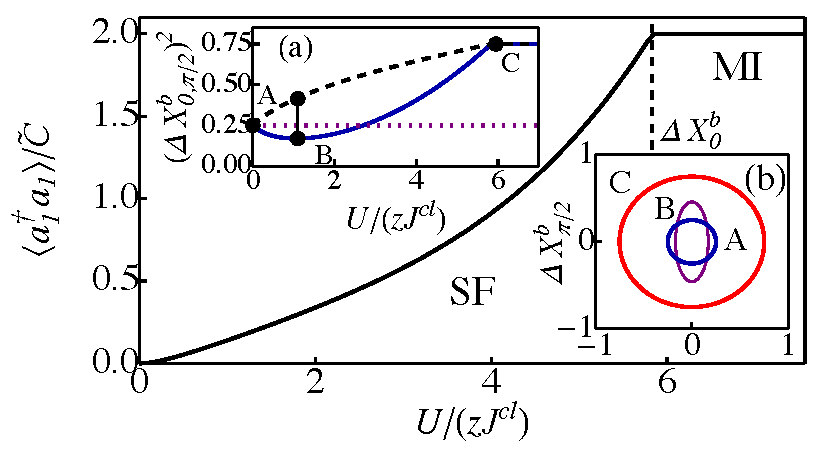
\includegraphics[width=\linewidth]{Quads}
  \captionsetup{justification=centerlast,font=small}
  \caption[Mean-Field Matter Quadratures]{Photon number scattered in a
    diffraction minimum, given by Eq. (\ref{intensity}), where
    $\tilde{C} = 2 |C|^2 (K-1) \mathcal{F}^2 [W_1](\pi/d)$.  More
    light is scattered from a MI than a SF due to the large
    uncertainty in phase in the insulator. (a) The variances of
    quadratures $\Delta X^b_0$ (solid) and $\Delta X^b_{\pi/2}$
    (dashed) of the matter field across the phase transition. Level
    1/4 is the minimal (Heisenberg) uncertainty. There are three
    important points along the phase transition: the coherent state
    (SF) at A, the amplitude-squeezed state at B, and the Fock state
    (MI) at C. (b) The uncertainties plotted in phase space.}
	\label{Quads}
\end{figure}

Probing $\hat{B}^2$ gives us access to kinetic energy fluctuations
with 4-point correlations ($\bd_i b_j$ combined in pairs). Measuring
the photon number variance, which is standard in quantum optics, will
lead up to 8-point correlations similar to 4-point density
correlations \cite{mekhov2007pra}. These are of significant interest,
because it has been shown that there are quantum entangled states that
manifest themselves only in high-order correlations
\cite{kaszlikowski2008}.

Surprisingly, inter-site terms scatter more light from a Mott
insulator than a superfluid Eq. \eqref{intensity}, as shown in
Fig. \eqref{Quads}, although the mean inter-site density
$\langle \hat{n}(\b{r})\rangle $ is tiny in a MI. This reflects a
fundamental effect of the boson interference in Fock states. It indeed
happens between two sites, but as the phase is uncertain, it results
in the large variance of $\hat{n}(\b{r})$ captured by light as shown
in Eq. \eqref{intensity}. The interference between two macroscopic
BECs has been observed and studied theoretically
\cite{horak1999}. When two BECs in Fock states interfere a phase
difference is established between them and an interference pattern is
observed which disappears when the results are averaged over a large
number of experimental realizations. This reflects the large
shot-to-shot phase fluctuations corresponding to a large inter-site
variance of $\hat{n}(\b{r})$. By contrast, our method enables the
observation of such phase uncertainty in a Fock state directly between
lattice sites on the microscopic scale in-situ.

\section{Conclusions}

In summary, we proposed a nondestructive method to probe quantum gases
in an optical lattice. Firstly, we showed that the density-term in
scattering has an angular distribution richer than classical
diffraction, derived generalized Bragg conditions, and estimated
parameters for the only two relevant experiments to date
\cite{weitenberg2011, miyake2011}. Secondly, we proposed how to
measure the matter-field interference by concentrating light between
the sites. This corresponds to interference at the shortest possible
distance in an optical lattice. By contrast, standard destructive
time-of-flight measurements deal with far-field interference and a
relatively near-field one was used in Ref. \cite{miyake2011}. This
defines most processes in optical lattices. E.g. matter-field phase
changes may happen not only due to external gradients, but also due to
intriguing effects such quantum jumps leading to phase flips at
neighbouring sites and sudden cancellation of tunneling
\cite{vukics2007}, which should be accessible by our method. In
mean-field, one can measure the matter-field amplitude (order
parameter), quadratures and squeezing. This can link atom optics to
areas where quantum optics has already made progress, e.g., quantum
imaging \cite{golubev2010, kolobov1999}, using an optical lattice as
an array of multimode nonclassical matter-field sources with a high
degree of entanglement for quantum information processing. Thirdly, we
demonstrated how the method accesses effects beyond mean-field and
distinguishes all the phases in the Mott-superfluid-glass transition,
which is currently a challenge \cite{derrico2014}. Based on
off-resonant scattering, and thus being insensitive to a detailed
atomic level structure, the method can be extended to molecules
\cite{LP2013}, spins, and fermions \cite{ruostekoski2009}.
